\documentclass[UTF-8]{ctexart}
\usepackage{ctex}
\usepackage[dvipsnames,svgnames]{xcolor}
\usepackage{newtxtext}
\usepackage{lipsum}
\usepackage[strict]{changepage}
\usepackage{framed}
\usepackage{graphicx}
\usepackage{float}
\usepackage{geometry}
\usepackage{amsmath}
\usepackage{tcolorbox}
\usepackage{amssymb}
\usepackage{mathrsfs}
\usepackage{cite}
\usepackage{bm}
\usepackage{listings}
\usepackage[colorlinks,linkcolor = Black]{hyperref}
\newcommand{\R}{\mathbb{R}}
\newcommand{\F}{\mathbb{F}}
\newcommand{\N}{\mathbb{N}}
\newcommand{\Q}{\mathbb{Q}}
\newcommand{\Z}{\mathbb{Z}}
\newcommand{\0}{\boldsymbol{0}}
\newcommand{\setparDis}{\setlength{\parskip} {0.3cm} }
\tcbuselibrary{most}
\definecolor{examplecolor}{rgb}{0.77,0.72,0.65} % 莫兰迪棕色
% ------------------******-------------------
\newtcolorbox{example}[2][]
{enhanced,breakable,
left=12pt,right=12pt,% 左右边距
% fonttitle=\bfseries, % 可以设置标题是否粗体
coltitle=white, % 标题字体颜色
colbacktitle=examplecolor, % 标题背景颜色
attach boxed title to top left={yshifttext=-1mm},
boxed title style={skin=enhancedfirst jigsaw,arc=1mm,bottom=0mm,boxrule=0mm},
boxrule=1pt, % 边框线宽
%
colback=OldLace, % 文本框背景颜色
colframe=examplecolor, % 框线颜色
%
sharp corners=northwest,
% drop fuzzy shadow, % 可以选择是否设置阴影效果
title=\vspace{3mm}#2,
arc=1mm,
#1}%

\newtcolorbox{justification}[2][]
{enhanced,breakable,
left=12pt,right=12pt,% 左右边距
% fonttitle=\bfseries, % 可以设置标题是否粗体
coltitle=white, % 标题字体颜色
colbacktitle=BurntOrange, % 标题背景颜色
attach boxed title to top left={yshifttext=-1mm},
boxed title style={skin=enhancedfirst jigsaw,arc=1mm,bottom=0mm,boxrule=0mm},
boxrule=1pt, % 边框线宽
%
colback=white, % 文本框背景颜色
colframe=BurntOrange, % 框线颜色
%
sharp corners=northwest,
% drop fuzzy shadow, % 可以选择是否设置阴影效果
title=\vspace{3mm}#2,
arc=1mm,
#1}%

\newtcolorbox{understanding}[2][]
{enhanced,breakable,
left=12pt,right=12pt,% 左右边距
% fonttitle=\bfseries, % 可以设置标题是否粗体
coltitle=white, % 标题字体颜色
colbacktitle=RoyalBlue, % 标题背景颜色
attach boxed title to top left={yshifttext=-1mm},
boxed title style={skin=enhancedfirst jigsaw,arc=1mm,bottom=0mm,boxrule=0mm},
boxrule=1pt, % 边框线宽
%
colback=white, % 文本框背景颜色
colframe=RoyalBlue, % 框线颜色
%
sharp corners=northwest,
% drop fuzzy shadow, % 可以选择是否设置阴影效果
title=\vspace{3mm}#2,
arc=1mm,
#1}%

\newtcolorbox{definition}[2][]
{enhanced,breakable,
left=12pt,right=12pt,% 左右边距
% fonttitle=\bfseries, % 可以设置标题是否粗体
coltitle=white, % 标题字体颜色
colbacktitle=Green, % 标题背景颜色
attach boxed title to top left={yshifttext=-1mm},
boxed title style={skin=enhancedfirst jigsaw,arc=1mm,bottom=0mm,boxrule=0mm},
boxrule=1pt, % 边框线宽
%
colback=white, % 文本框背景颜色
colframe=Green, % 框线颜色
%
sharp corners=northwest,
% drop fuzzy shadow, % 可以选择是否设置阴影效果
title=\vspace{3mm}#2,
arc=1mm,
#1}%
\definecolor{blueshade}{rgb}{0.95,0.95,1} % 蓝色文本框,竖线颜色设为 RoyalBlue
\definecolor{greenshade}{rgb}{0.90,0.99,0.91} % 绿色文本框,竖线颜色设为 Green
\definecolor{redshade}{rgb}{1.00,0.90,0.90}% 红色文本框,竖线颜色设为 LightCoral
\definecolor{brownshade}{rgb}{0.99,0.97,0.93} % 棕色文本框,竖线颜色设为 BurlyWood


\newenvironment{brownformal}{%
\def\FrameCommand{%
\hspace{1pt}%
{\color{BurlyWood}\vrule width 2pt}%
{\color{brownshade}\vrule width 4pt}%
\colorbox{brownshade}%
}%
\MakeFramed{\advance\hsize-\width\FrameRestore}%
\noindent\hspace{-4.55pt}% disable indenting first paragraph
\begin{adjustwidth}{}{7pt}%
\vspace{2pt}\vspace{2pt}%
}
{%
\vspace{2pt}\end{adjustwidth}\endMakeFramed%
}

\newenvironment{blueformal}{%
\def\FrameCommand{%
\hspace{1pt}%
{\color{RoyalBlue}\vrule width 2pt}%
{\color{blueshade}\vrule width 4pt}%
\colorbox{blueshade}%
}%
\MakeFramed{\advance\hsize-\width\FrameRestore}%
\noindent\hspace{-4.55pt}% disable indenting first paragraph
\begin{adjustwidth}{}{7pt}%
\vspace{2pt}\vspace{2pt}%
}
{%
\vspace{2pt}\end{adjustwidth}\endMakeFramed%
}

\newtheorem{thm}{定理}

\lstset{
    basicstyle          =   \sffamily,          % 基本代码风格
    keywordstyle        =   \bfseries,          % 关键字风格
    commentstyle        =   \rmfamily\itshape,  % 注释的风格,斜体
    stringstyle         =   \ttfamily,  % 字符串风格
    flexiblecolumns,                % 别问为什么,加上这个
    numbers             =   left,   % 行号的位置在左边
    showspaces          =   false,  % 是否显示空格,显示了有点乱,所以不现实了
    numberstyle         =   \zihao{-5}\ttfamily,    % 行号的样式,小五号,tt等宽字体
    showstringspaces    =   false,
    captionpos          =   t,      % 这段代码的名字所呈现的位置,t指的是top上面
    frame               =   lrtb,   % 显示边框
}


\hypersetup{
colorlinks = true,
linkcolor = Black,
filecolor = Black,
bookmarks = true,
urlcolor = RoyalBlue,
citecolor = cyan,
bookmarksopen = false,
pdfpagemode = FullScreen,
pdfstartview = Fit
}

\CTEXsetup[format={\bfseries}]{section}
\CTEXsetup[format={\bfseries}]{subsection}
\begin{document}
\begin{titlepage}
    \centering

    %------------------------------------------------------------
    %    Top rules
    %------------------------------------------------------------

    \rule{\textwidth}{1pt}   % The top horizontal rule
    \vspace{0.2\textheight}  % Whitespace between top horizontal rule and title

    %------------------------------------------------------------
    %    Title
    %------------------------------------------------------------

    {\Huge \kaishu  符号计算改良的分析化学计算方法}

    \vspace{0.01\textheight}

    {\huge \kaishu 对NaHA酸碱度的分析}

    \vspace{0.025\textheight}   % Whitespace between the title and short horizontal rule

    \rule{0.83\textwidth}{0.4pt}  % The short horizontal rule under title

    \vspace{0.1\textheight}  % Whitespace between the short horizontal rule and author

    %------------------------------------------------------------
    %    Author
    %------------------------------------------------------------

    {\Large \textsc{\kaishu 禤科材}}

    \vspace{0.015\textheight}

    {\Large \textsc{\kaishu 中国科学技术大学\;化学物理系}}

    \vfill  % Whitespace between author and date

    {\large \kaishu 2022年3月3日}
    \vspace{0.1\textheight}  % Whitespace between date and bottom horizontal rule

    %------------------------------------------------------------
    %    Bottom rules
    %------------------------------------------------------------

    \rule{\textwidth}{1pt}  % The bottom horizontal rule

  \end{titlepage}
\setparDis
\nocite{*}
\begin{abstract}
    \kaishu \fontsize{10pt}{16pt}
        两性物质 $\text{NaHA} $溶液的  $\text{PH}$  计算是分析化学的重要内容。教科书介绍了多种 $\text{PH} $近似公式,但各公式的适用条件一度缺少详细论证,且目前仍然处于争论之中。本文以 $\text{Mathematica}$ 符号计算软件为辅助,发扬了分析化学去公式化计算方法。针对学术界一直头疼的$ \text{NaHA}$ 酸碱度计算公式的选择问题,作者利用数学分析方法及可视化手段,深刻揭示了各公式的可行域空间,力求为分析化学师生彻底扫除障碍。
    \end{abstract}
\tableofcontents

\pagebreak

    \kaishu \fontsize{11pt}{16pt}
\section{引言}
二元弱酸 $\text{H}_2\text{A}$ 的酸式盐 $\text{NaHA} $为两性物质。在浓度为 $c$ 的 $\text{NaHA} $溶液中有以下关系:
\begin{enumerate}
    \item 电荷守恒: $[Na^+]+[H^+]=[HA^-]+2[A^{2-}]+[OH^-] $
    \item 物料守恒: $[Na^+]=[H_2A]+[HA^-]+[A^{2-}] $
    \item 一级电离: $K_1=\frac{[H^+][HA^-]} {[H_2A]} $
    \item 二级电离: $K_2=\frac{[H^+][A^{2-}]} {[HA^-]} $
\end{enumerate}
为了简化计算,引入分析浓度 $c$  (A的总浓度)与分布分数(组分占有 $c$ 的比例):
\begin{align*} 
    [H_2A]&=c*\frac{[H^+]^2} {[H^+]^2+[H^+]K_1+K_1K_2}       \\ 
    [HA^-]&=c*\frac{[H^+]K_1} {[H^+]^2+[H^+]K_1+K_1K_2}       \\ 
    [A^{2-}]&=c*\frac{K_1K_2} {[H^+]^2+[H^+]K_1+K_1K_2}       
\end{align*}

将上述组分浓度代入电荷守恒,得到关于氢离子浓度$ [H^+] $的高次多项式方程:
\begin{equation} \label{基本方程}
    c+[H^+]= \frac{[H^+]K_1+2K_1K_2} {[H^+]^2+[H^+]K_1+K_1K_2} +\frac{K_w}{[H^+]}
\end{equation}
其中 $K_w$ 为水的离子积常数,此处默认常温下 $K_w=10^{-14}$ 。对于给定的二元酸式盐 $\text{NaHA}$ ,已知两级电离常数 $K_1$ 和 $K_2$ ,给定浓度 $c$  ,求解上述方程即可得知此时氢离子浓度的准确值(忽略离子活度)。但由于上述方程求解不便,传统分析化学的处理方法为引入近似条件,将氢离子浓度$ [H^+] $化简为显函数形式。以下是经典教科书中给出的四个近似公式及其适用条件:
\begin{align*}      
    [H_{x1}]&= \sqrt{     \frac{K_1(c *K_2+Kw)}  {c+K_1} }\;&c&\geq500K_2\\   
    [H_{x2}]&= \sqrt{     \frac{K_1(c *K_2)}  {c+K_1} }     &c&\geq500K_2 \;\&\&\;K_{2}c\geq20K_w \\     
    [H_{x3}]&= \sqrt{     K_1K_2 } &c&\geq20K_1\\   
    [H_{x4}]&= \sqrt{     \frac{K_1(c *K_2+Kw)}  {c} } &c&\geq500K_2\;\&\&\;K_{2}c\geq20K_w
\end{align*} 
  
  传统体系“记忆换运算,近似换简化”的思路同学们都不陌生。然而,这样的近似公式会造成学习上的不便甚至混淆:
  {\fontsize{10pt}{16pt} \begin{enumerate}
      \item 一些公式的适用范围存在交集,实际应用中究竟哪一个公式适用区间更普遍?
      \item 适用的边界条件究竟如何与 物理意义(二级电离、水的电离)相联系?
  \end{enumerate}}

  在计算机高度发达的今天,我们可以很轻易地解诸如(\ref{基本方程})这样的方程,传统近似手段简化运算的价值正逐渐丧失。并且,如何真正完备地刻画使用公式带来的误差以及它们的适用范围,成为目前去公式化方法和传统体系之间的主要矛盾。为此,本文以 $\text{Mathematica}$ 为平台,充分运用数学、计算机手段,讨论近似公式的可行域区间,推动分析化学课程的发展。
  
\section{数学准备}
\subsection{可行域}
由于 $[H^+]$、$K_1$、$K_2$,$c$ 数值非常小,对它们取负对数之后, $PH$、$PK_1$、$PK_2$、$Pc$ 四个变量满足的关系如下:
\begin{align*}     
    PH_1&=-\log_{10} \sqrt{     \frac{10^{-PK_1}(10^{-Pc} *10^{-PK_2}+Kw)}  {10^{-Pc}+10^{-PK_1}} }\\  PH_2&= -\log_{10} \sqrt{     \frac{10^{-PK_1}(10^{-Pc} *10^{-PK_2})}  {10^{-Pc}+10^{-PK_1}} }\\      PH_3&=-\log_{10} \sqrt{     10^{-PK_1}*10^{-PK_2} }\\   PH_4&=-\log_{10} \sqrt{     \frac{10^{-PK_1}(c *10^{-PK_2}+Kw)}  {10^{-Pc}} } 
\end{align*}
引入相空间 $\R^3=\{\;\bm{x}= (PK_1,PK_2,Pc)\;|\;PK_1,PK_2,Pc\in \R\;\}$ 以描述已知的三个初始条件。如此一来,四大公式可看作 $\R^3\rightarrow  \R,(\bm{x}\;\rightarrow \;PH)$ 一个映射。

\textcolor{RoyalBlue}{\textbf{我们的目的,在于找出所有满足“相对准确值误差在$5\%$以内”的三维点所构成的集合}}。由函数的连续性可知,它是一个连通集。以相对氢离子准确值误差 $5\% $为标准,设 $PH$ 准确值为 $F(\bm{x}),\bm{x} = (PK_1,PK_2,Pc)$ ,定义误差函数 $\Delta (\bm{x}),\bm{x}\in \R^3 $。简单推导可知,$ \Delta(\bm{x})=|\;f_i(\bm{x})-F(\bm{x})\;|\leq0.02 $即为所求区域满足的限制条件。我们称不等式的解集为\textcolor{RoyalBlue}{\textbf{可行域}}。

\begin{definition}{Definition:可行域}
    \kaishu \fontsize{11pt}{16pt}
    称$\R^n$中的一个区域$S^n$为近似公式$f$的可行域,如果
    \[
        \forall \bm{x} = (x_1,x_2,\dots,x_n) \in S^n, |\;f(\bm{x})-F(\bm{x})\;|\leq0.02 
    \]
    其中$F(\bm{x})$为物理量的理论准确值。
\end{definition}

\vspace{0.02\textheight} 

\begin{figure}[ht]
    \centering
    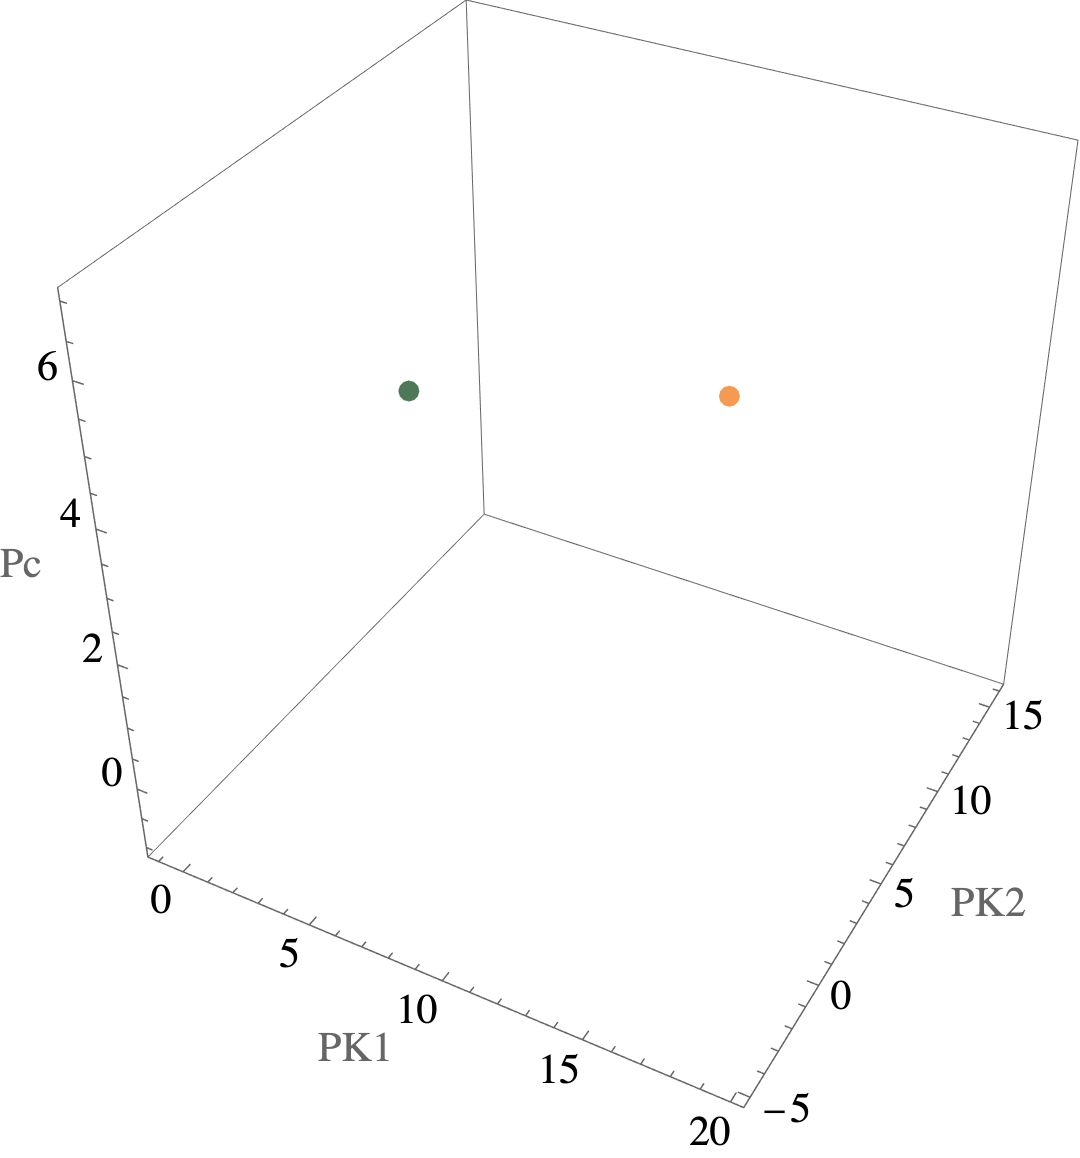
\includegraphics[width=0.7\textwidth]{映射.jpg}
    \caption{\kaishu 相空间中两个点分别对应两个PH值}
    \label{fig:映射}
\end{figure}

\subsection{对数变换}
将这一对应关系写作:
\begin{align*}    
    f_1(PK_1, PK_2, Pc)&=-\log_{10} \sqrt{     \frac{10^{-PK_1}(10^{-Pc} *10^{-PK_2}+Kw)}  {10^{-Pc}+10^{-PK_1}} } \\
    f_2(PK_1, PK_2, Pc)&= -\log_{10} \sqrt{     \frac{10^{-PK_1}(10^{-Pc} *10^{-PK_2})}  {10^{-Pc}+10^{-PK_1}} } \\
    f_3(PK_1,PK_2,Pc)&=-\log_{10} \sqrt{     10^{-PK_1}*10^{-PK_2} }\\  
    f_4(PK_1,PK_2,Pc)&=-\log_{10} \sqrt{     \frac{10^{-PK_1}(10^{-Pc} *10^{-PK_2}+Kw)}  {10^{-Pc}} }\\ 
\end{align*}
由数学分析知识可知,所有满足条件的点,在相空间中分布于边界曲面的同一侧。对原方程(\ref{基本方程})作对数变换:
\begin{equation} \label{对数变换}
    10^{-Pc}+10^{-PH}= \frac{10^{-PH}10^{-PK_1}+2*10^{-PK_1}10^{-PK_2}} {10^{-2PH}+10^{-PH}10^{-PK_1}+10^{-PK_1}10^{-PK_2}} +\frac{K_w}{10^{-PH}} 
\end{equation}
几乎无法表示为$ PH $关于$ PK_1$、$PH_2$、$Pc$ 的显函数,误差函数 $\Delta (\bm{x})$ 难于推导。故退而寻求数值解。

\section{线性近似公式的解析与讨论}
\subsection{作图}
公式$[H_{x3}]$经对数变换后的形式较为简单——$PH $关于 $PK_1$ 和 $PK_2 $具有线性性质,在新的相空间 $\R^3=\{\;\bm{y}= (PK_1,PK_2,PH)\;|\;PK_1,PK_2,PH\in R\;\} $中的图像是一张平面:
\begin{equation*}   
    PH=\frac12PK_1+\frac12PK_2 
\end{equation*}

在相空间 $\R^3=\{\;\bm{y}= (PK_1,PK_2,PH)\;|\;PK_1,PK_2,PH\in R\;\} $中,满足与精确酸度方程(\ref{对数变换})误差$ 0.02$ 的两张曲面分别是:

{\fontsize{9pt}{16pt} 
\begin{align}
    10^{-Pc}+10^{-(PH-0.02)}&= \frac{10^{-(PH-0.02)}10^{-PK_1}+2*10^{-PK_1}10^{-PK_2}} {10^{-2(PH-0.02)}+10^{-(PH-0.02)}10^{-PK_1}+10^{-PK_1}10^{-PK_2}} +\frac{K_w}{10^{-(PH-0.02)}}\\
    10^{-Pc}+10^{-(PH+0.02)}&= \frac{10^{-(PH+0.02)}10^{-PK_1}+2*10^{-PK_1}10^{-PK_2}} {10^{-2(PH+0.02)}+10^{-(PH+0.02)}10^{-PK_1}+10^{-PK_1}10^{-PK_2}} +\frac{K_w}{10^{-(PH+0.02)}}
\end{align}
}

与$PH=\frac12PK_1+\frac12PK_2 $联立消去$PH$,即得$\R^3$中关于$(PK_1,PK_2,Pc)$的方程
{\fontsize{9pt}{14pt}
\begin{align*}
    10^{-Pc}+10^{-(\frac12PK_1+\frac12PK_2 -0.02)}&= \frac{10^{-(\frac12PK_1+\frac12PK_2 -0.02)}10^{-PK_1}+2*10^{-PK_1}10^{-PK_2}} {10^{-2(\frac12PK_1+\frac12PK_2 -0.02)}+10^{-(\frac12PK_1+\frac12PK_2 -0.02)}10^{-PK_1}+10^{-PK_1}10^{-PK_2}} \\
    &+ \frac{K_w}{10^{-(\frac12PK_1+\frac12PK_2 -0.02)}} \\
    10^{-Pc}+10^{-(\frac12PK_1+\frac12PK_2 +0.02)}&= \frac{10^{-(\frac12PK_1+\frac12PK_2 +0.02)}10^{-PK_1}+2*10^{-PK_1}10^{-PK_2}} {10^{-2(\frac12PK_1+\frac12PK_2 +0.02)}+10^{-(\frac12PK_1+\frac12PK_2 +0.02)}10^{-PK_1}+10^{-PK_1}10^{-PK_2}} \\
    &+\frac{K_w}{10^{-(\frac12PK_1+\frac12PK_2 +0.02)}}
\end{align*}
}
对应的曲面即是可行域的边界。分别记作$ \text{sup}\,(\bm{x}) $和$ \text{inf}\,(\bm{x}) $,作图如下:

\begin{figure}[ht]
    \centering
    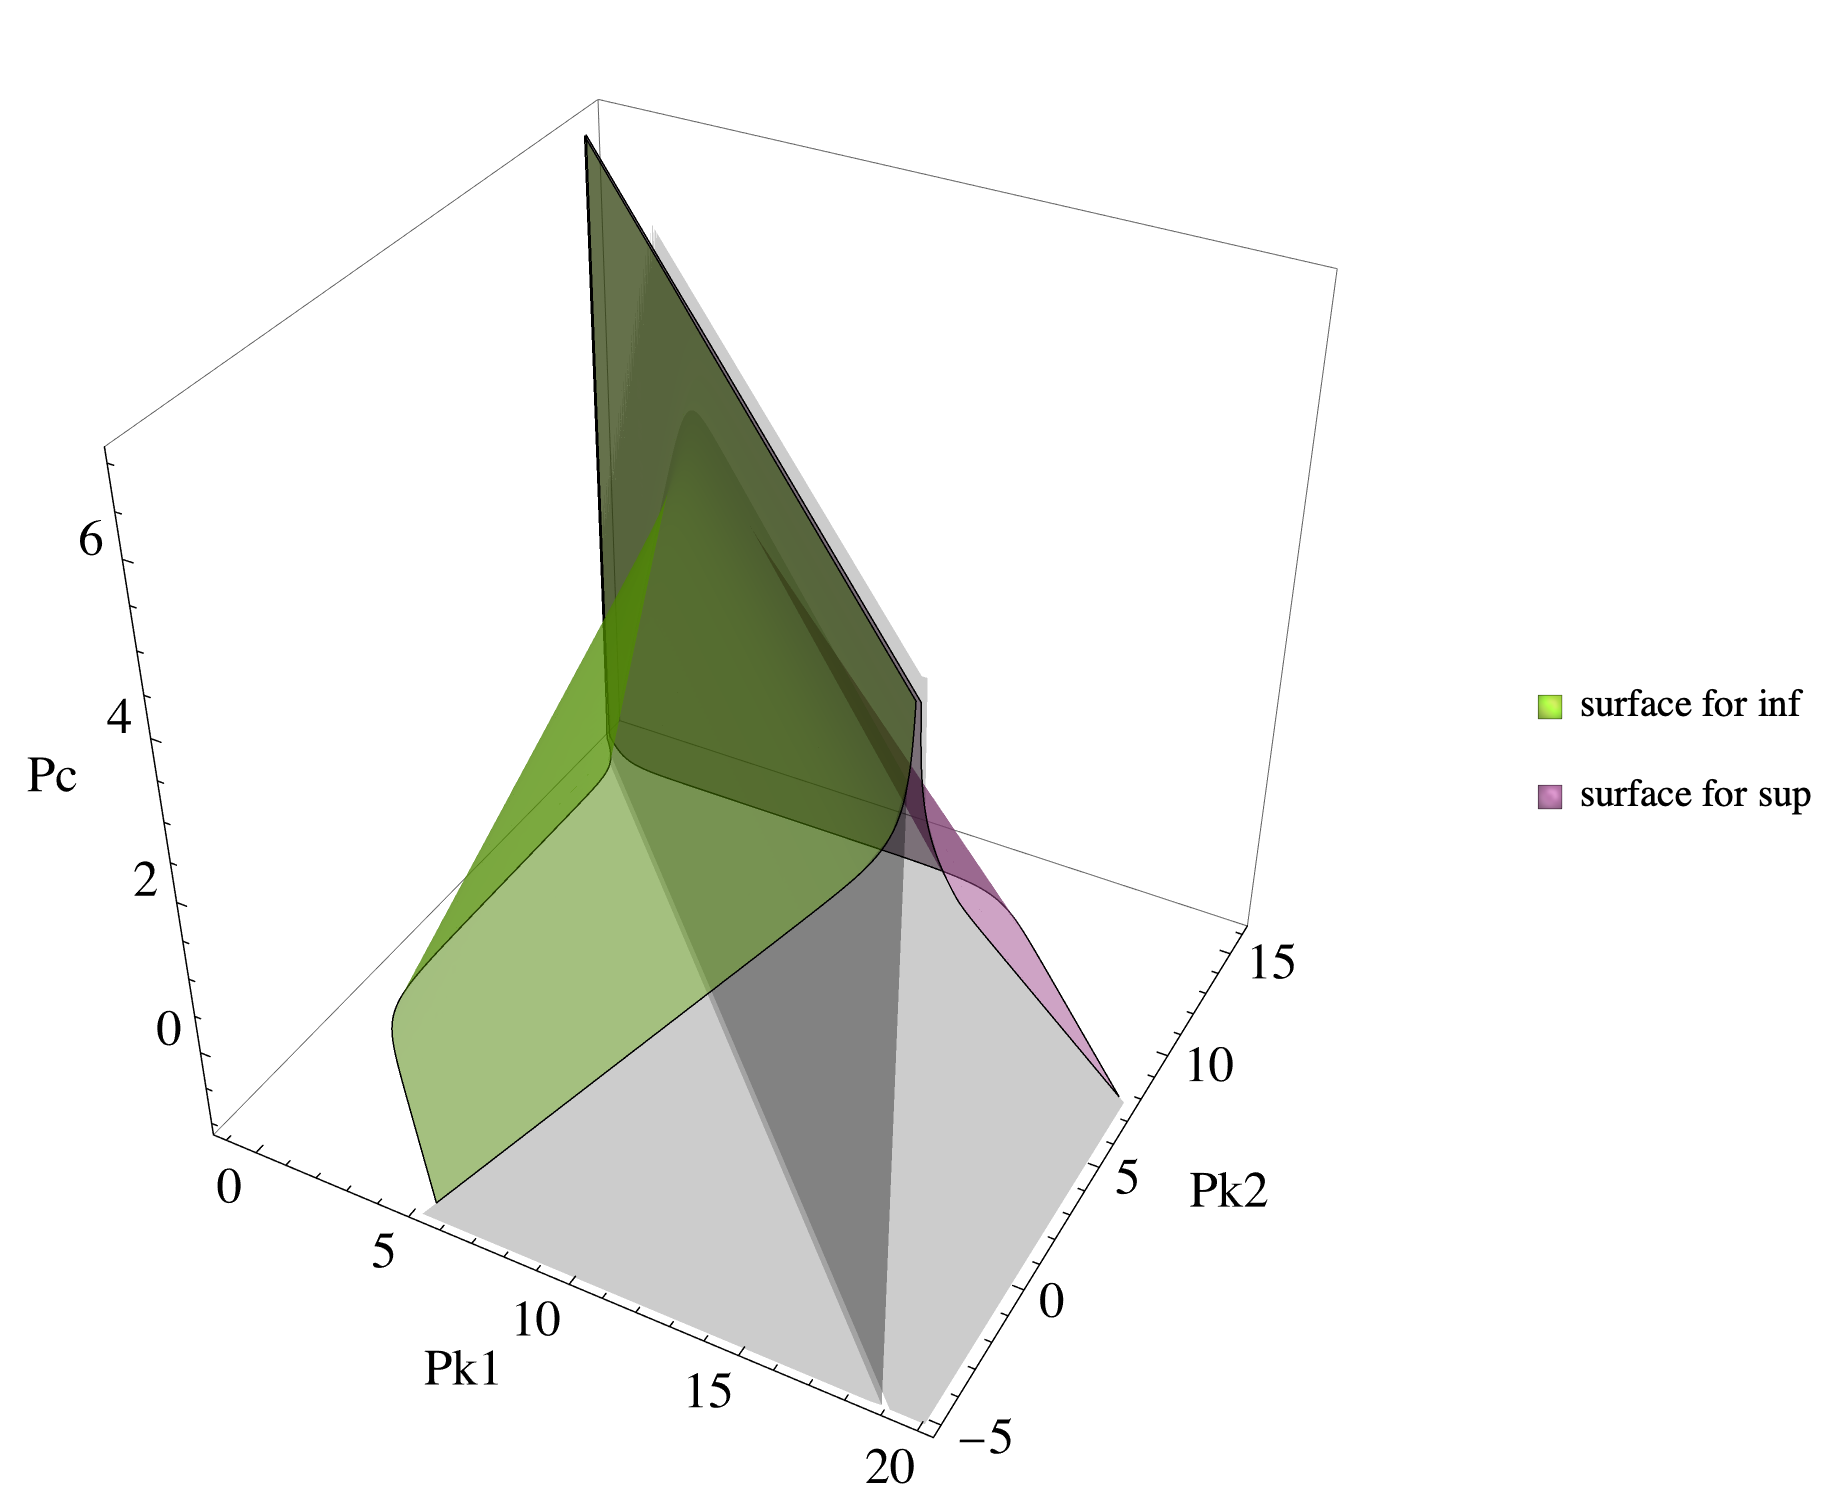
\includegraphics[width=0.7\textwidth]{完整.png}
    \caption{\kaishu 可行域}
    \label{fig:完整}
\end{figure}

可行域就是图中的阴影区域。

\subsection{讨论}
公式 $f_3$ 的秘密已经一览无余。比如固定$Pc=2$,误差函数 
\[
    \Delta (PK_1,PK_2,2)=|\; f_3(PK_1,PK_2,2)-F(PK_1,PK_2,2)\;|
\]
的解为 $\R^2$ 的子集,是可行域在$Pc=2$处的截面:

\begin{figure}[ht]
    \centering
    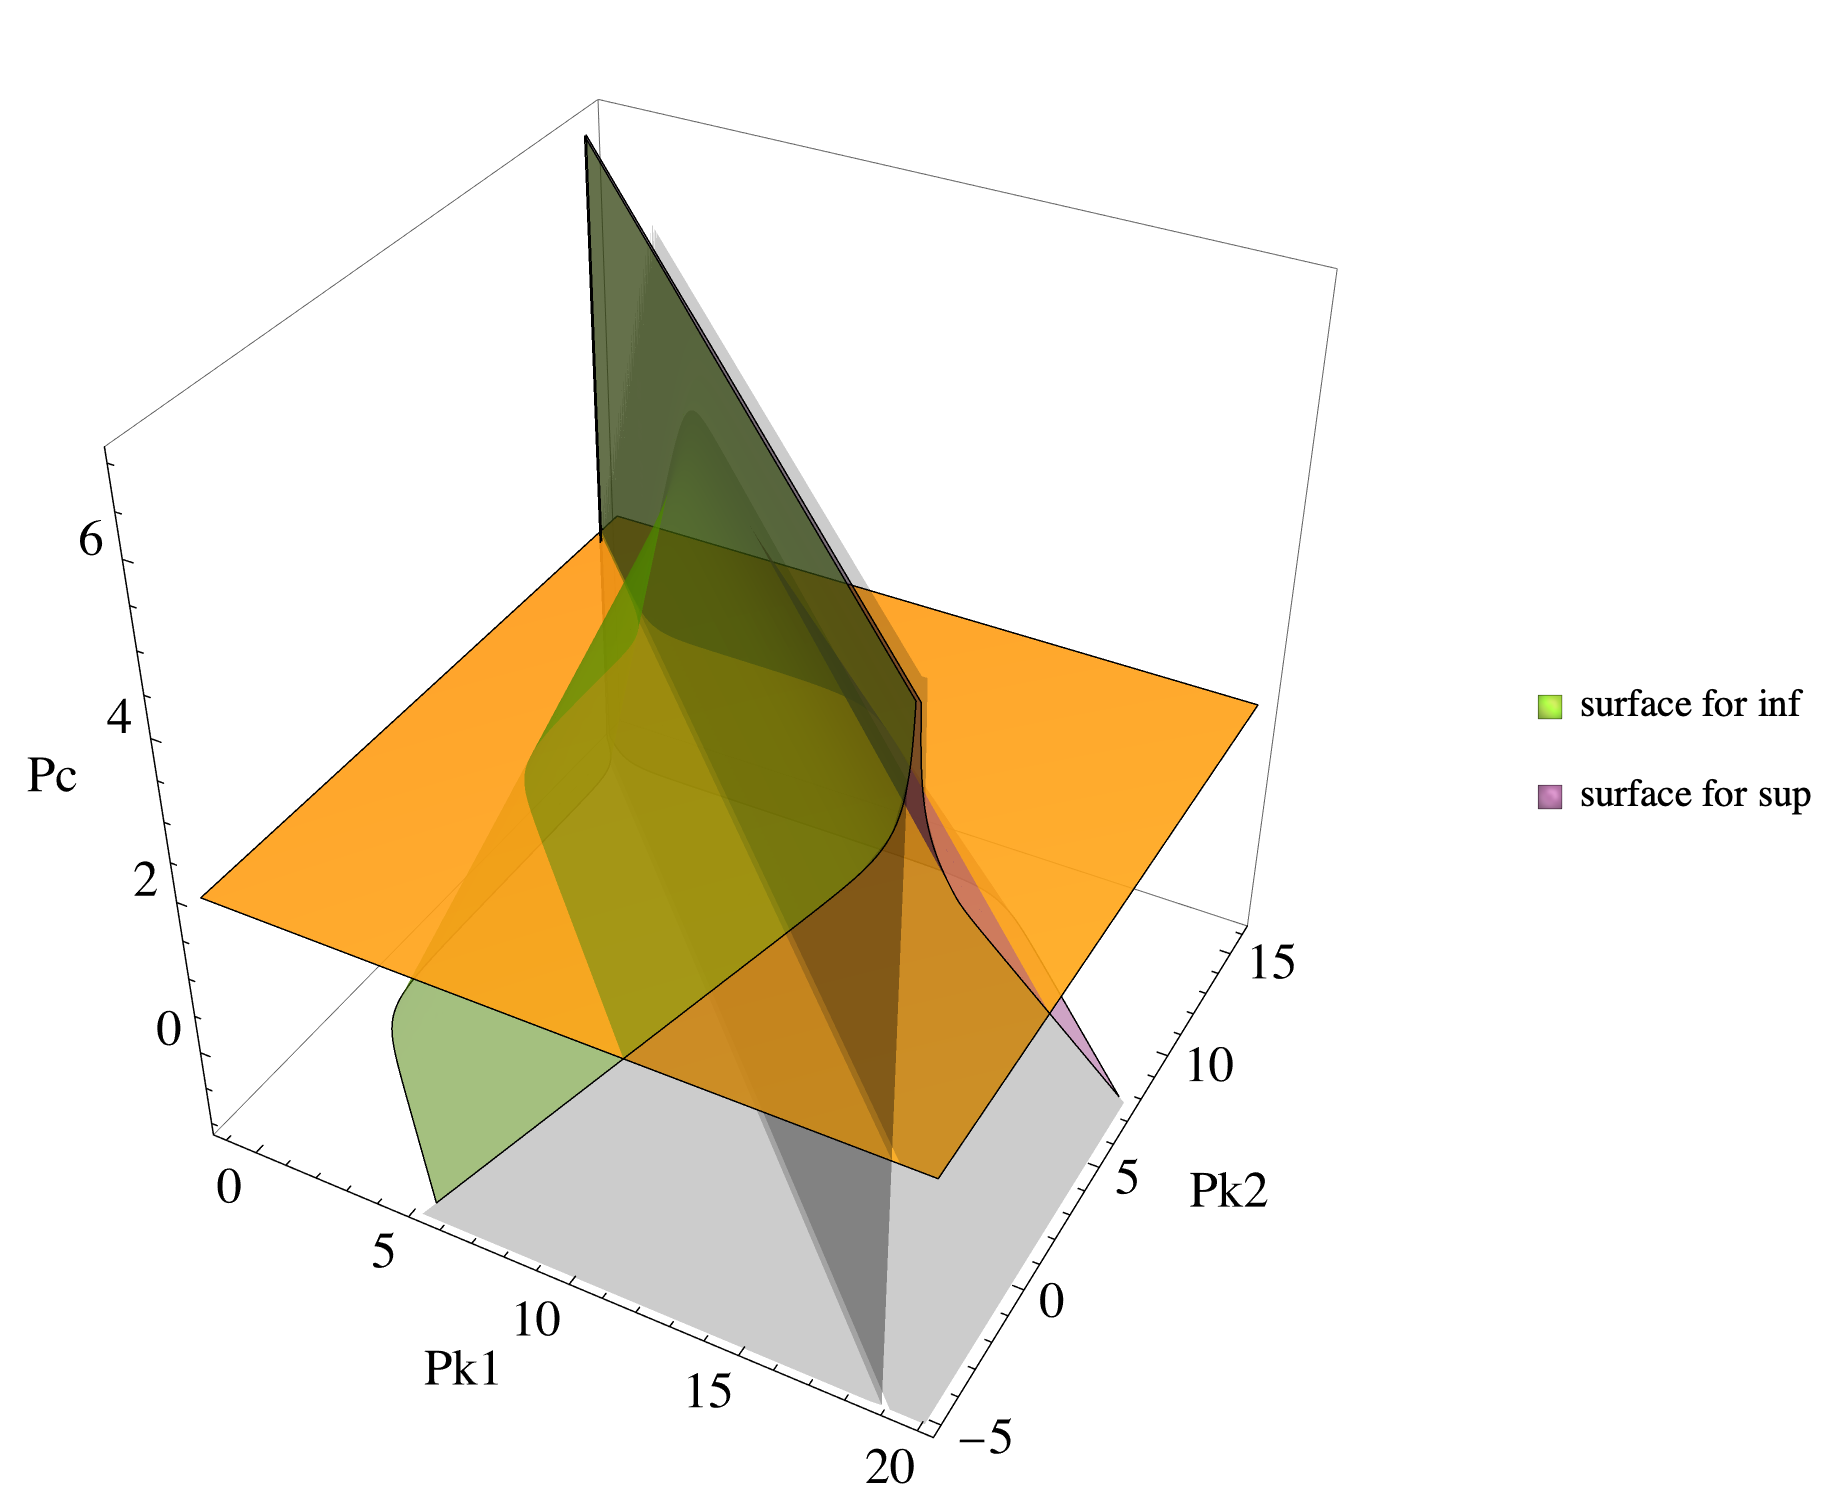
\includegraphics[width=0.9\textwidth]{截面.png}
    \caption{\kaishu 可行域的截面}
    \label{fig:截面}
\end{figure}

又如,对公式的适用条件
\begin{align*}     
        &c\geq500K_2\;\;\;\;\; &\text{condition} \;1\\   
        &c\geq500K_2 \;\&\&\;K_{2}c\geq20K_w &\text{condition}\;2\\    
        &c\geq20K_1   &\text{condition}\;3
\end{align*}
作对数变换得
\begin{align*}     
Pc&\leq\log (500)PK_2 \;\;\;\;\;&\text{condition} \;1\\ 
Pc+PK_2&\leq\log (20)K_w &\text{condition}\;2\\
Pc&\leq\log (20)PK_1 &\text{condition}\;3
\end{align*}
可见变换后的结果都描述了相空间$ \R^3=\{\;\bm{x}= (PK_1,PK_2,Pc)\;|\;PK_1,PK_2,Pc\in R\;\}$ 中一个以平面为边界的区域。将它们和完整的可行域放在一起考虑:

\begin{figure}[ht]
    \centering
    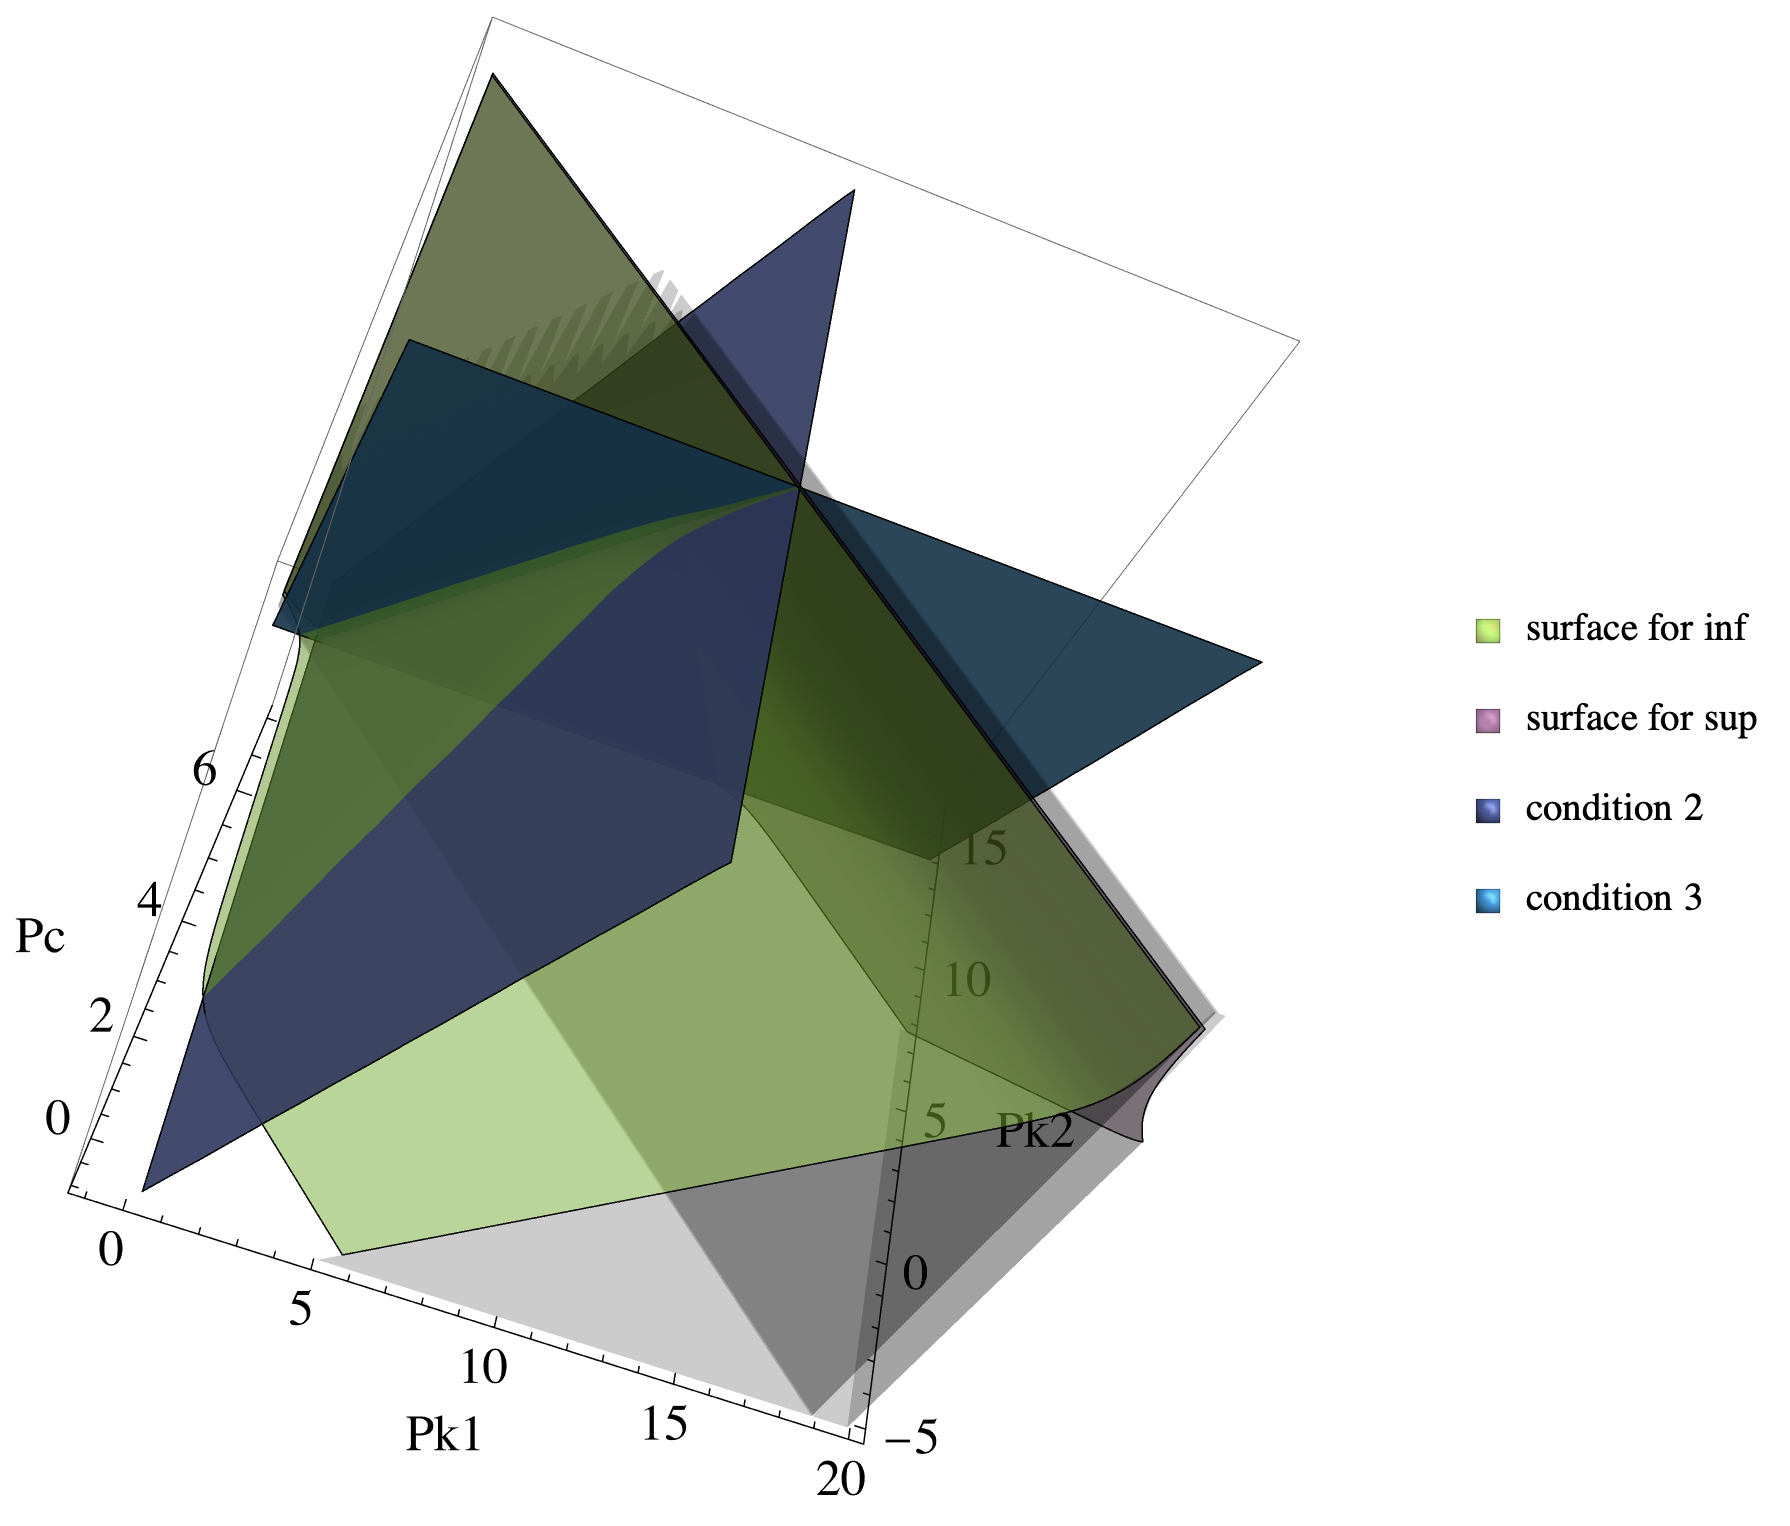
\includegraphics[width=0.8\textwidth]{封面.png}
    \caption{\kaishu 可行域与传统适用条件}
    \label{fig:可行域与传统适用条件}
\end{figure}

可见这些限制都具有一定的局限性。现今对于传统条件中 $20$ 、 $500$ 等位置的常数更准确的研究即可简化为:\textcolor{RoyalBlue}{\textbf{寻找可行域边界曲面的最优二元线性拟合函数}}——在本文提出完整可行域(图\ref{fig:完整})之后便可迎刃而解。在此,作者建议用 $10.365$来替代条件$ Pc+PK_2\geq\log (20)K_w $ 中原本“ $20$ ”的位置。

代码附于文末,读者可自行尝试。

\section{其他公式}
\subsection{其他可行域}
不难从以上步骤总结出研究计算可行域的一般方法:对数变换$ \Rightarrow $ 刻画误差$ \Rightarrow $消去 $PH$ $\Rightarrow $作图。如法炮制,易得四大公式可行域的边界如下:

\begin{figure}[ht]
    \centering
    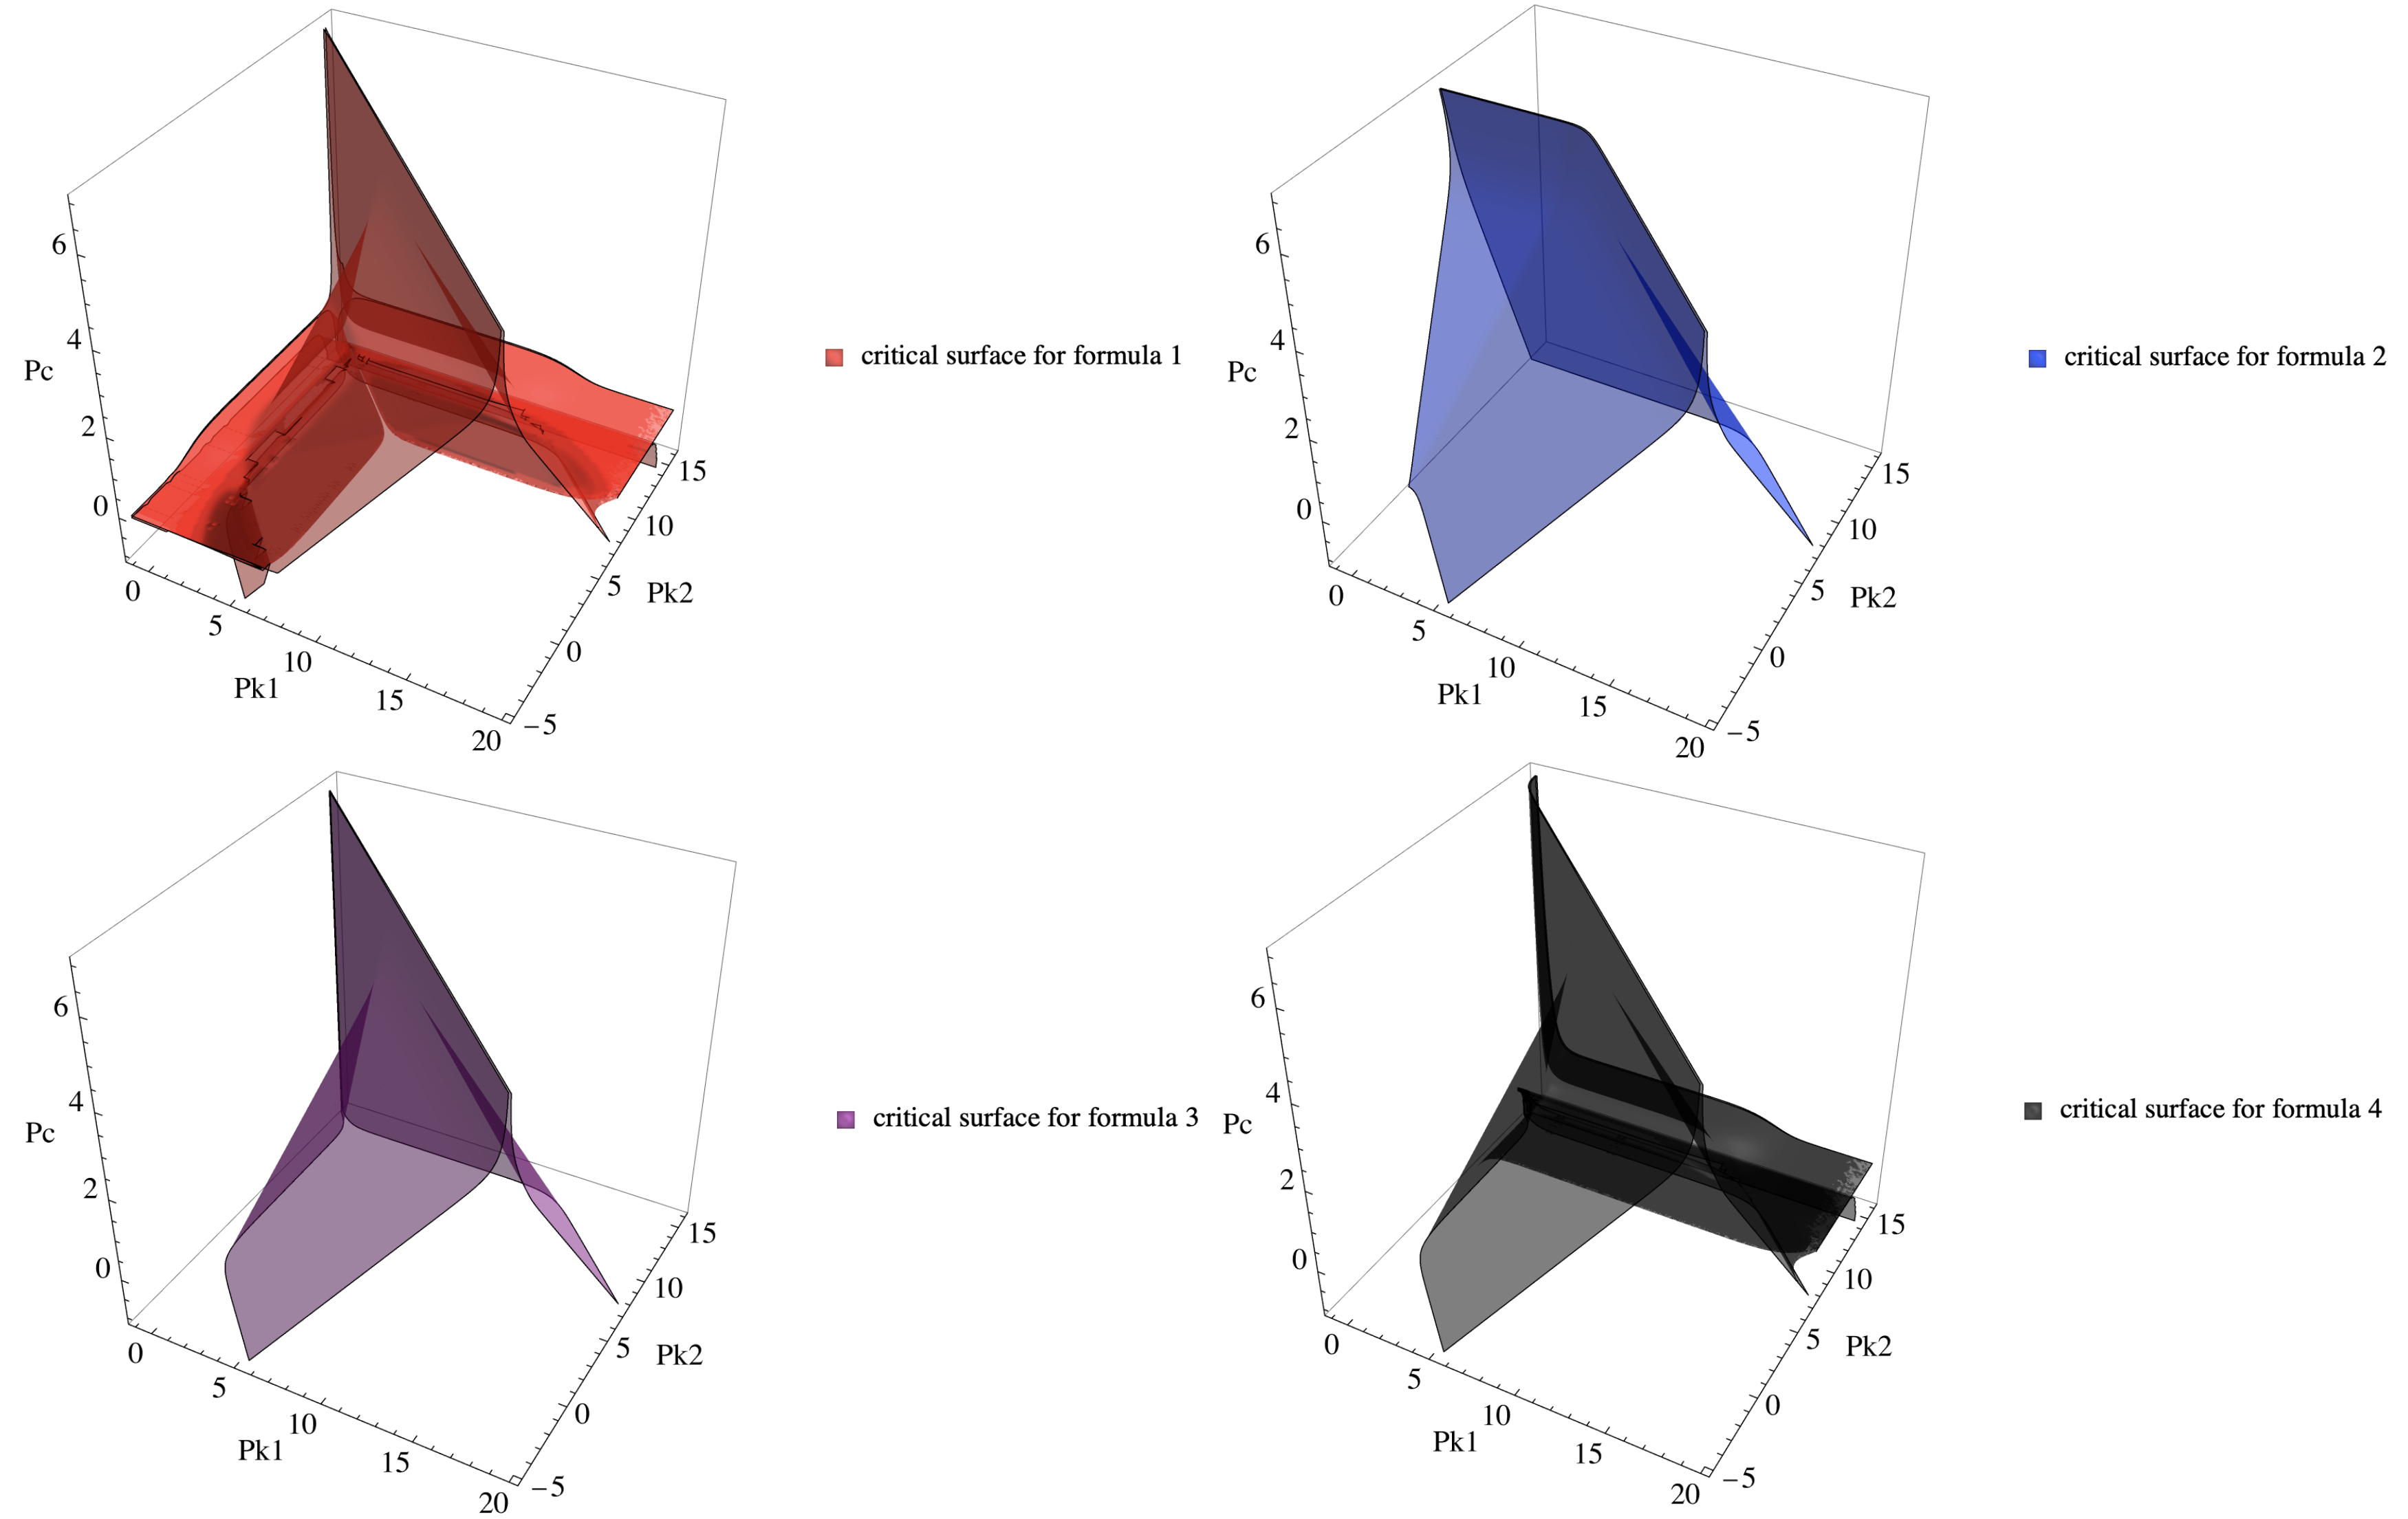
\includegraphics[width=0.8\textwidth]{四大.png}
    \caption{\kaishu 四大近似公式的可行域}
    \label{fig:四大}
\end{figure}
结合公式$f_3$的经验以及可行域的实际物理意义,读者不难判断可行域的位置。可以发现,在分析浓度小于$10^{-6}$的区间,四大公式基本完全失效。

\subsection{最优近似}
由于计算能力的不足,前人对于“哪一个公式在给定误差下的可行域最广?”的问题难以给出明确的回答。然而在计算系统高度发达的当下,找出这一最优公式已是易如反掌。我们借助可视化手段,将四大公式的可行域边界分别重叠(图\ref{fig:12}),可见公式
\[
    [H]_{x_2}= \sqrt{     \frac{K_1(c *K_2)}  {c+K_1} }
\]
对应的可行域最为宽广。在误差不大于$5\%$的标准下的优越性一目了然。

\section{结论}
本文以相对精确结果 $[H^+]$ 偏差 $5\% $为标准,使用数学方法和计算机手段,引入描述已知条件的 $\R^3 $相空间,深刻揭示了 $\text{NaHA} $酸碱度四大近似公式的可行域。希望能为分析化学师生彻底扫除认知障碍。

对于具体公式的选择问题上,基于可行域空间最宽广的原则,公式
\[
[H]= \sqrt{     \frac{K_1(c *K_2)}  {c+K_1} }
\]
是其中最优。虽然其他公式有一定的物理意义,但实际效果并不大,剔除之无大碍。

对于形如 $\text{Na}_m\text{H}_n\text{A}$ 的更多元酸式盐,已知条件是 $m+n+1 $维向量$ (PK_1\dots,PK_n,Pc) $,可行域的边界曲面将在高维空间中展开。本文的方法虽然在原则上仍然适用,但略显复杂,需要更多的线性代数知识来辅助处理。如果过程过于复杂,可以参考 EDTA 配位滴定金属离子的处理方式,引入“表观浓度”以简化运算。

\textcolor{RoyalBlue}{\textbf{交流电和生物电是两种不同的资源,它们应当各得其所}}。用计算机手段求解化学平衡问题,一定是分析化学课程教学改革的发展方向。

\section{鸣谢}
本文写作得到了中国科学技术大学化学系邵利民副教授的鼎力支持。

面对一些困难,刘毅凡同学为作者提供了很多帮助和鼓励。

此外还有来自四面八方的建议,在此一并感谢!

\pagebreak

\section{部分代码与附图}
    $c = 0.1$下的精确$PH$:
    \begin{lstlisting}
        c = 0.1;
        accurate = 
        ContourPlot3D[
        c + 10^-PH == kw/10^-PH + c ((10^-PH*10^-Pk1 + 2*10^-Pk1*10^-Pk2)/
        (10^(-2 PH) + 10^-PH*10^-Pk1 + 10^-Pk1*10^-Pk2)), {Pk1, 0, 20}, 
        {Pk2, 0, 20}, {PH, 0, 14},PlotTheme -> "Scientific", AxesLabel -> 
        Automatic, AxesStyle -> Directive[14], PlotLegends -> {"accurate PH"}, 
        PlotRange -> Full]
    \end{lstlisting}

    特定浓度可行域:
    \begin{lstlisting}
        c = 0.1;
        cp3sup = 
        Table[{FindRoot[{c + 10^-(PH - 0.02) == 
        kw/10^-(PH - 0.02) + c ((10^-(PH - 0.02)*10^-Pk1 + 2*10^-Pk1*10^-Pk2)/(
        10^(-2 (PH - 0.02)) + 10^-(PH - 0.02)*10^-Pk1 + 10^-Pk1*10^-Pk2)), 
        PH == 1/2 Pk1 + 1/2 Pk2, Pk2 == a}, {Pk1, 20}, {Pk2, a}, {PH, 20}, 
        WorkingPrecision -> MachinePrecision][[1, 2]], a}, {a, 0, 14, 0.05}];
        
        cp3supline = 
        ListLinePlot[cp3sup, PlotTheme -> "Detailed", PlotStyle -> Orange, 
        FrameLabel -> {{HoldForm[Pk2], None}, {HoldForm[Pk1], None}}, 
        PlotLabel -> HoldForm[c = 0.1 M时公式 Subscript[H, x3] 的可行域], 
        LabelStyle -> {15, GrayLevel[0]}];

        cp3inf = 
        Table[{FindRoot[{c + 10^-(PH + 0.02) == 
        kw/10^-(PH + 0.02) + c ((10^-(PH + 0.02)*10^-Pk1 + 2*10^-Pk1*10^-Pk2)/(
        10^(-2 (PH + 0.02)) + 10^-(PH + 0.02)*10^-Pk1 + 10^-Pk1*10^-Pk2)), 
        PH == 1/2 Pk1 + 1/2 Pk2, Pk2 == a}, {Pk1, 20}, {Pk2, a}, {PH, 20}, 
        WorkingPrecision -> MachinePrecision][[1, 2]], a}, {a, 0, 14, 0.05}];

        cp3infline = 
        ListLinePlot[cp3inf, PlotTheme -> "Detailed", PlotStyle -> Orange, 
        FrameLabel -> {{HoldForm[Pk2], None}, {HoldForm[Pk1], None}}, 
        PlotLabel -> HoldForm[c = 0.1 M时公式 Subscript[H, x3] 的可行域], 
        LabelStyle -> {15, GrayLevel[0]}];

        Show[cp3supline, cp3infline, 
        Graphics[{Thick, Dashed, Orange, Line[{cp3inf[[1]], cp3sup[[1]]}]}], 
        AspectRatio -> 1]
    \end{lstlisting}

    完整可行域:
    \begin{lstlisting}
        cp3infsurface = 
        ContourPlot3D[
        10^-Pc + 10^-(1/2 Pk1 + 1/2 Pk2 + 0.02) == kw/10^-(1/2 Pk1 + 1/2 Pk2 
        + 0.02) + 10^-Pc*((10^-(1/2 Pk1 + 1/2 Pk2 + 0.02)*10^-Pk1 + 
        2*10^-Pk1*10^-Pk2)/(10^(-2 (1/2 Pk1 + 1/2 Pk2 + 0.02)) + 
        10^-(1/2 Pk1 + 1/2 Pk2 + 0.02)*10^-Pk1 + 
        10^-Pk1*10^-Pk2)), {Pk1, -1, 20}, {Pk2, -5, 16}, {Pc, -1, 7}, 
        ContourStyle -> {RGBColor[0.5355579515419151, 0.9430131641554946, 
        0.004882822085237493], Opacity[0.5]}, ImageSize -> {500, 500}, 
        AxesLabel -> Automatic, AxesStyle -> Directive[Black, 17], 
        PlotLegends -> {"surface for inf"}, PlotRange -> Full, 
        PlotTheme -> "Scientific", Mesh -> None];

        cp3supsurface = 
        ContourPlot3D[
        10^-Pc + 10^-(1/2 Pk1 + 1/2 Pk2 - 0.02) == 
        kw/10^-(1/2 Pk1 + 1/2 Pk2 - 0.02) + 
        10^-Pc*((10^-(1/2 Pk1 + 1/2 Pk2 - 0.02)*10^-Pk1 + 2*10^-Pk1*10^-Pk2)/
        (10^(-2 (1/2 Pk1 + 1/2 Pk2 - 0.02)) + 10^-(1/2 Pk1 + 1/2 Pk2 - 0.02)
        *10^-Pk1 + 10^-Pk1*10^-Pk2)), {Pk1, -1, 20}, {Pk2, -5, 16}, {Pc, -1, 7}, 
        ContourStyle -> {RGBColor[0.5864078175768783, 0.26359194937432395`,
        0.519486597936422], Opacity[0.5]}, ImageSize -> {500, 500}, 
        AxesLabel -> Automatic, AxesStyle -> Directive[Black, 17], 
        PlotLegends -> {"surface for sup"}, PlotRange -> Full, 
        PlotTheme -> "Scientific", Mesh -> None];

        shadow3inf = 
        Plot3D[-Log10[(kw/10^-(1/2 Pk1 + 1/2 Pk2 + 0.02) - 
        10^-(1/2 Pk1 + 1/2 Pk2 + 0.02))/(1 - ((10^-(1/2 Pk1 + 1/2 
        Pk2 + 0.02)*10^-Pk1 + 2*10^-Pk1*10^-Pk2)/(10^(-2 (1/2 Pk1 + 1/2 Pk2 + 0.02)) 
        + 10^-(1/2 Pk1 + 1/2 Pk2 + 0.02)*10^-Pk1 + 
        10^-Pk1*10^-Pk2)))], {Pk1, -1, 20}, {Pk2, -5, 16}, 
        PlotStyle -> Directive[RGBColor[0.5355579515419151, 0.9430131641554946, 
        0.004882822085237493], Opacity[0]], Filling -> Bottom, Mesh -> None, 
        BoundaryStyle -> None];

        shadow3sup = 
        Plot3D[-Log10[(kw/10^-(1/2 Pk1 + 1/2 Pk2 - 0.02) - 
        10^-(1/2 Pk1 + 1/2 Pk2 - 0.02))/(1 - ((10^-(1/2 Pk1 + 1/2 Pk2 - 0.02)
        *10^-Pk1 + 2*10^-Pk1*10^-Pk2)/(
        10^(-2 (1/2 Pk1 + 1/2 Pk2 - 0.02)) + 
        10^-(1/2 Pk1 + 1/2 Pk2 - 0.02)*10^-Pk1 + 
        10^-Pk1*10^-Pk2)))], {Pk1, -1, 20}, {Pk2, -5, 16}, 
        PlotStyle -> Directive[RGBColor[0.5864078175768783, 0.26359194937432395`,
        0.519486597936422], Opacity[0]], Filling -> Bottom, Mesh -> None, 
        BoundaryStyle -> None];

        Show[cp3infsurface, cp3supsurface, shadow3inf, shadow3sup]
    \end{lstlisting}

   

\pagebreak

\begin{figure}[ht]
    \centering
    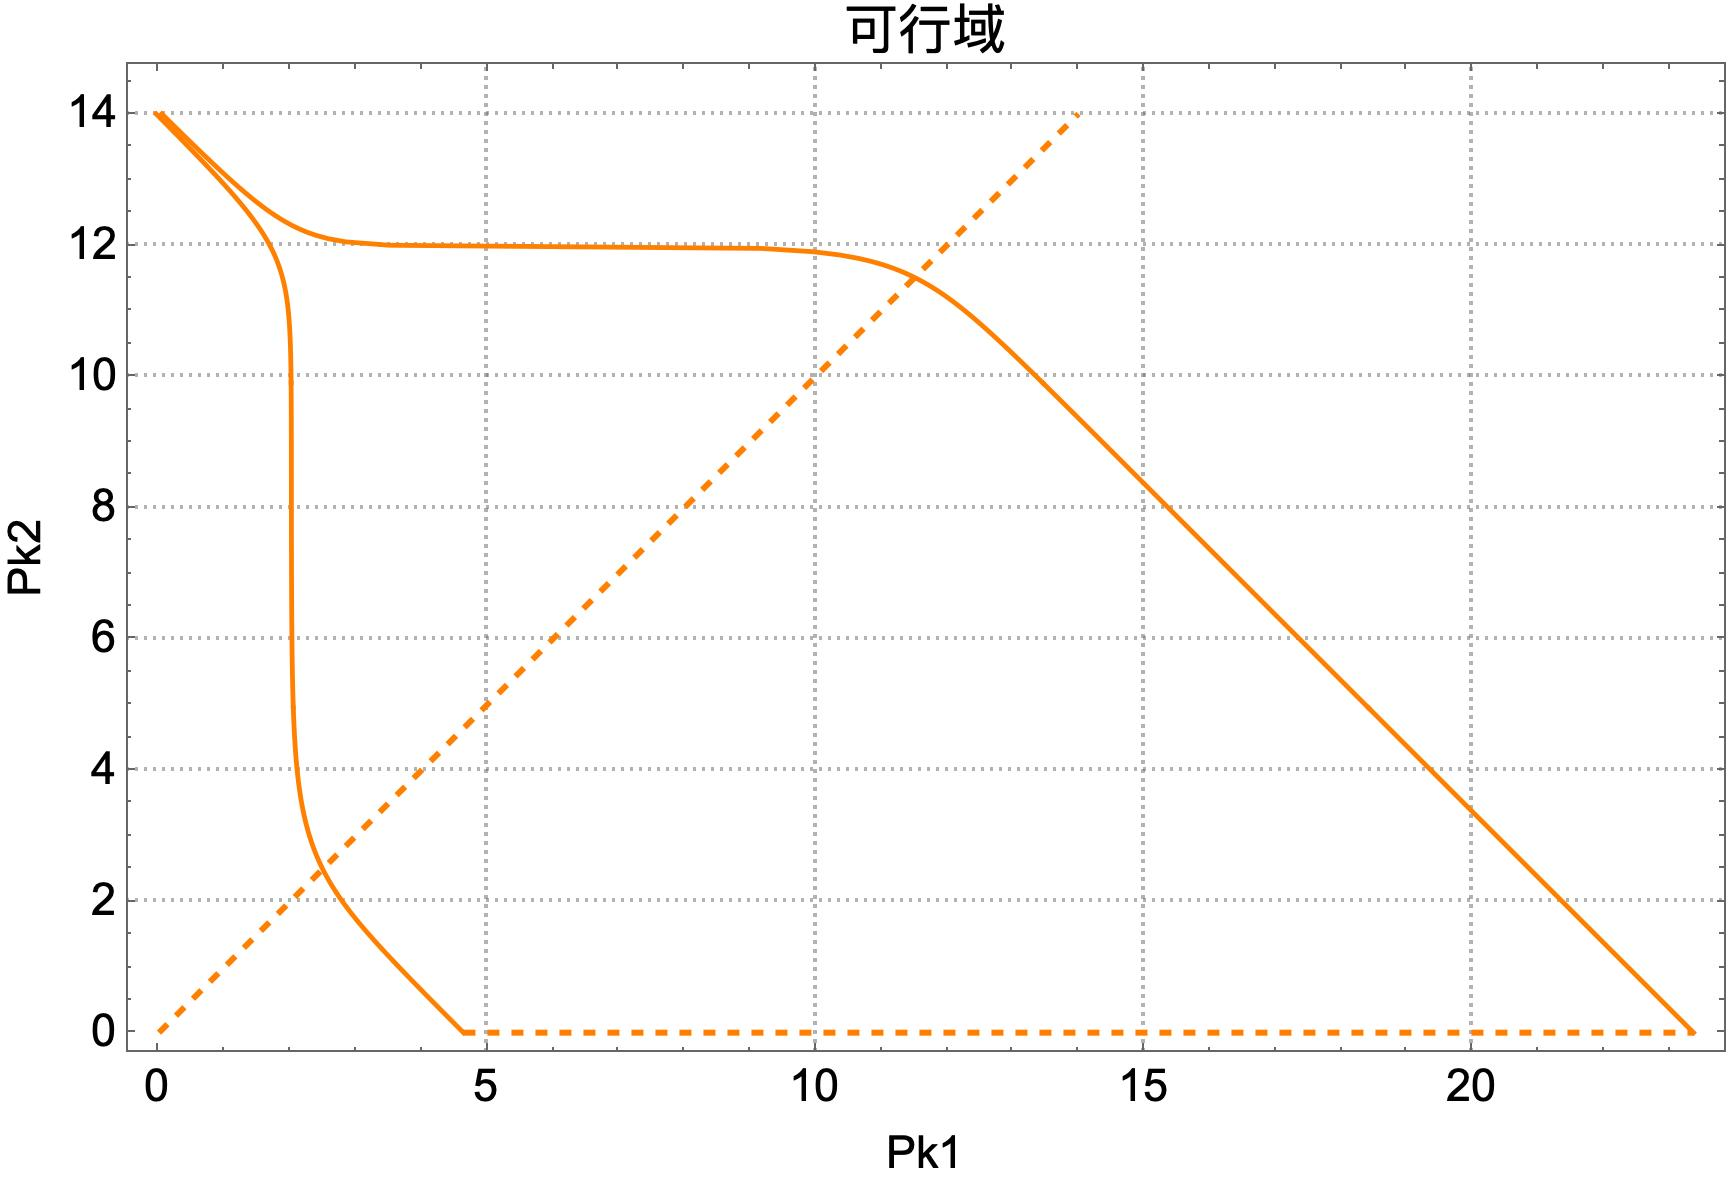
\includegraphics[width=0.8\textwidth]{截面a.jpeg}
    \caption{\kaishu PH = 2时可行域截面}
    \label{fig:截面a}
\end{figure}

\begin{figure}[ht]
    \centering
    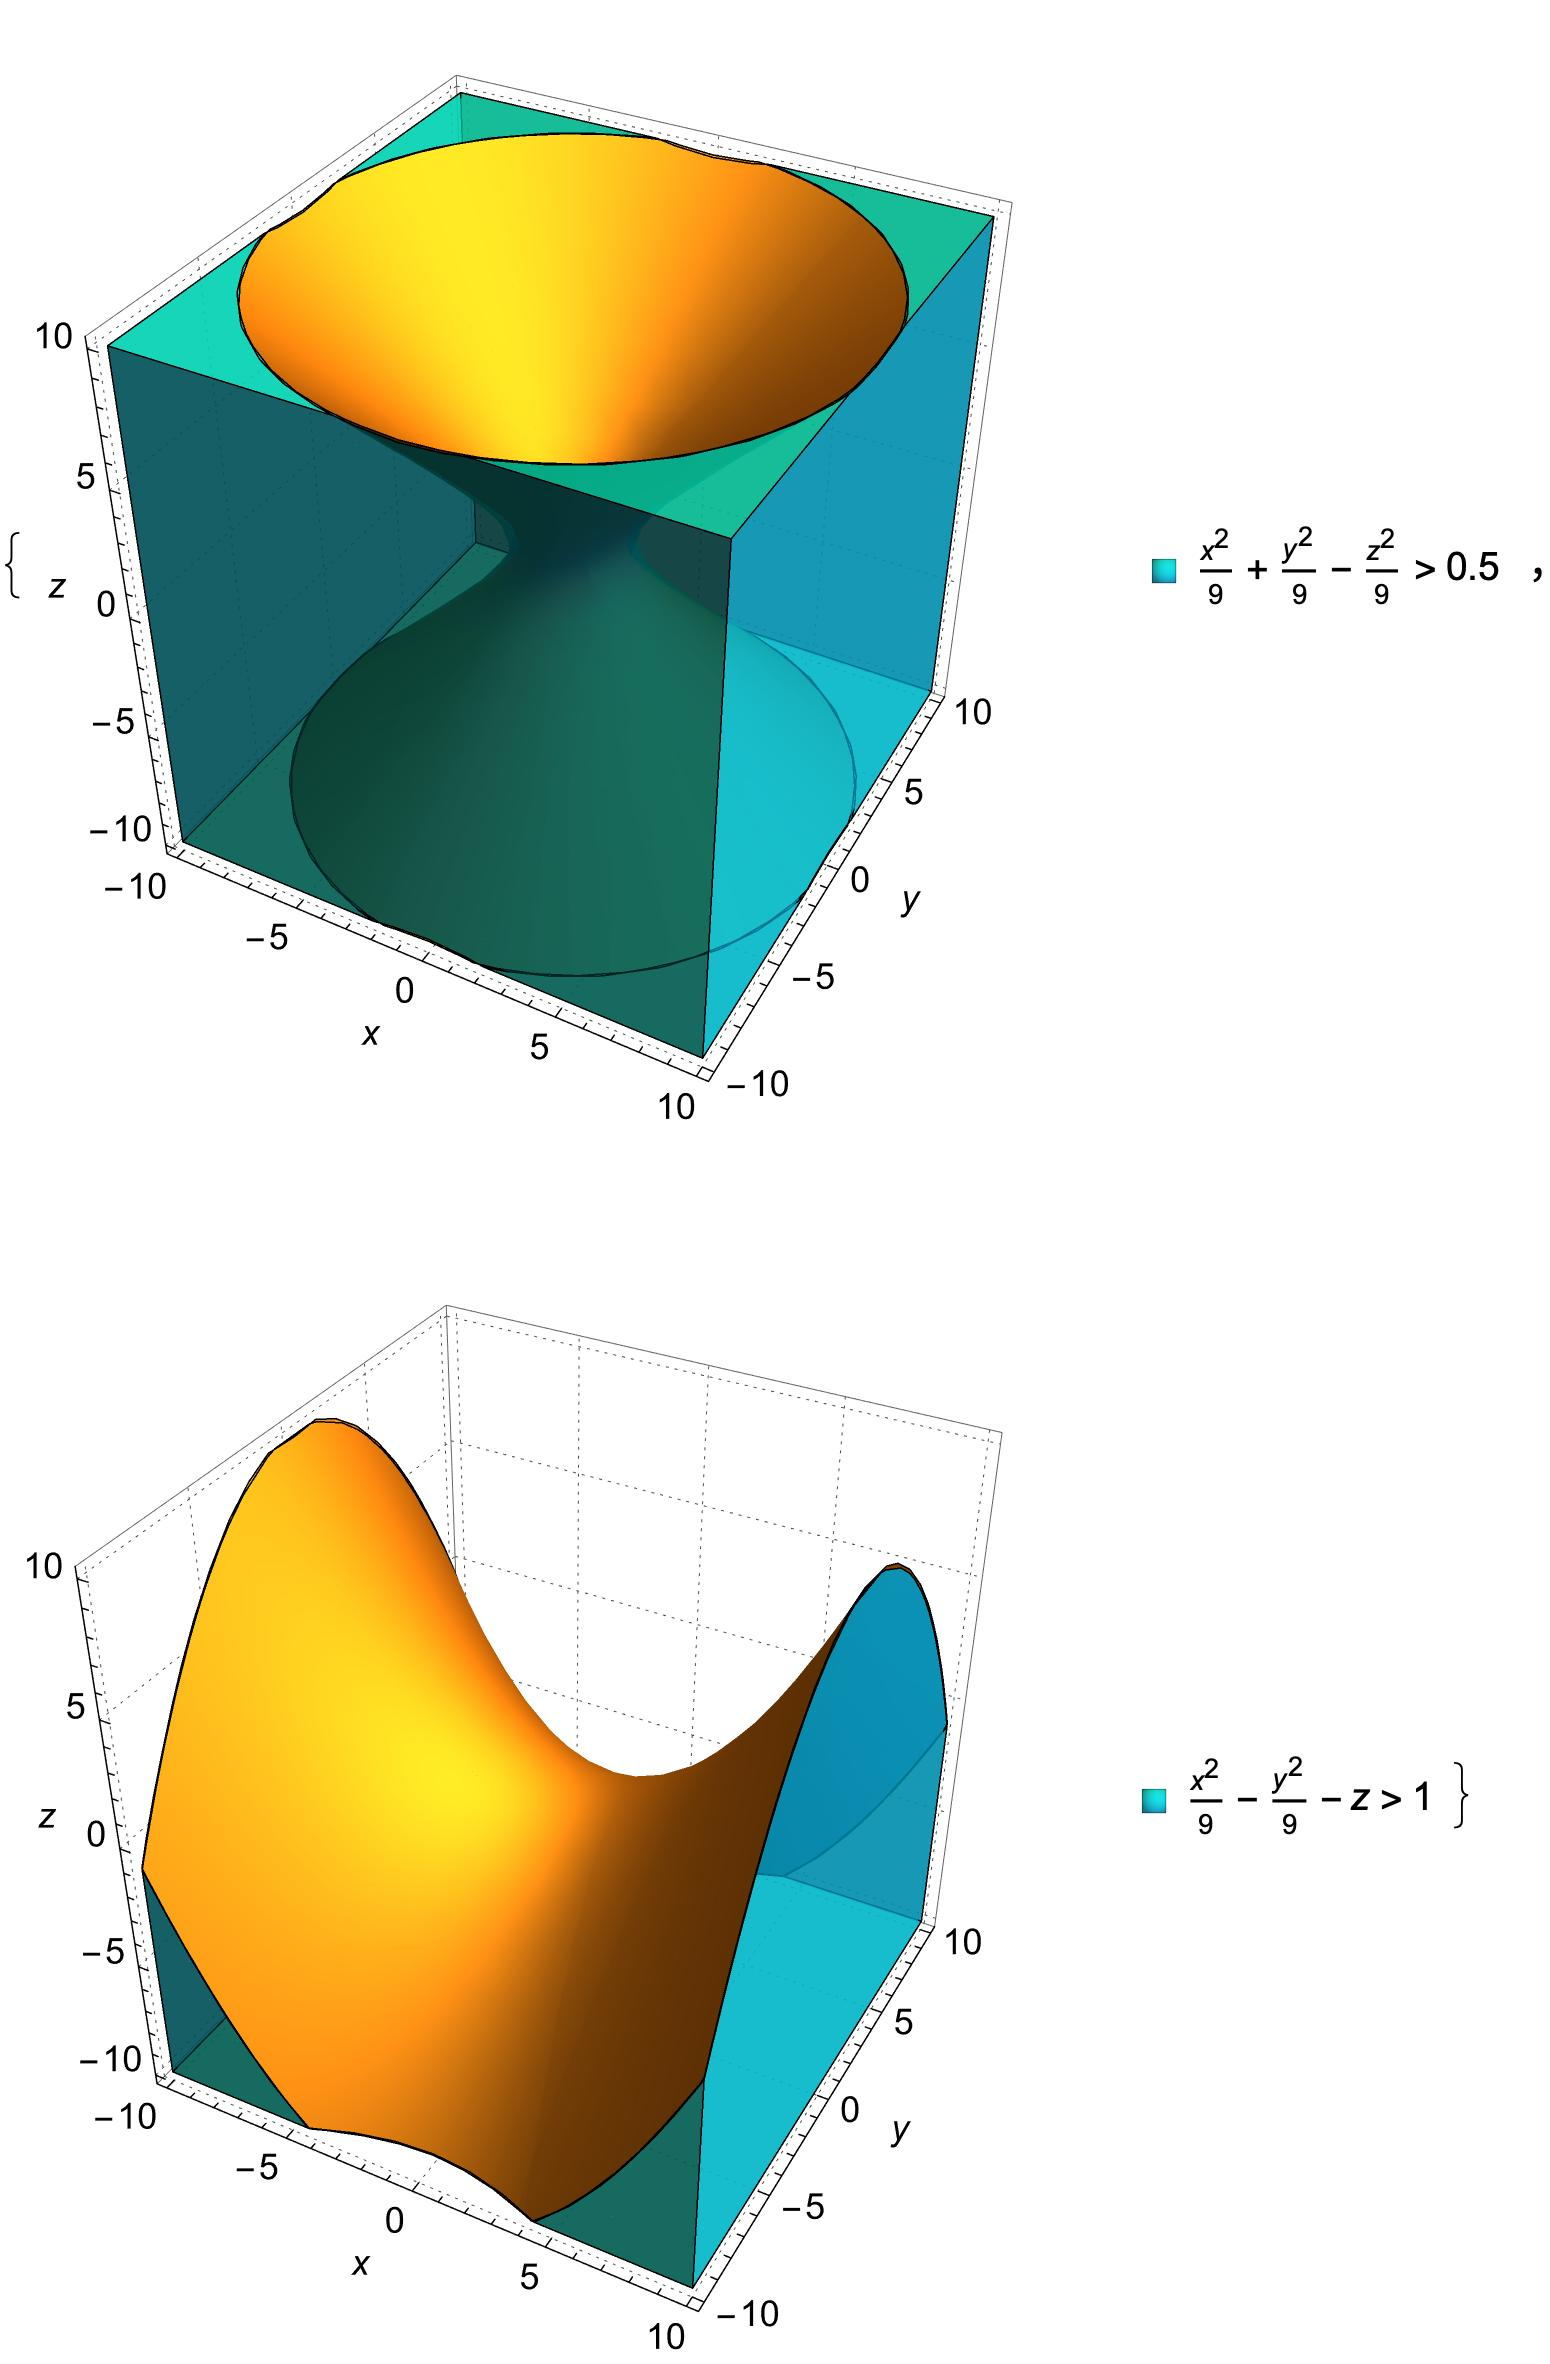
\includegraphics[width=0.8\textwidth]{双曲面.jpeg}
    \caption{\kaishu 以单叶抛物面和马鞍面为边界的区域}
    \label{fig:边界区域}
\end{figure}

\begin{figure}
    \centering
    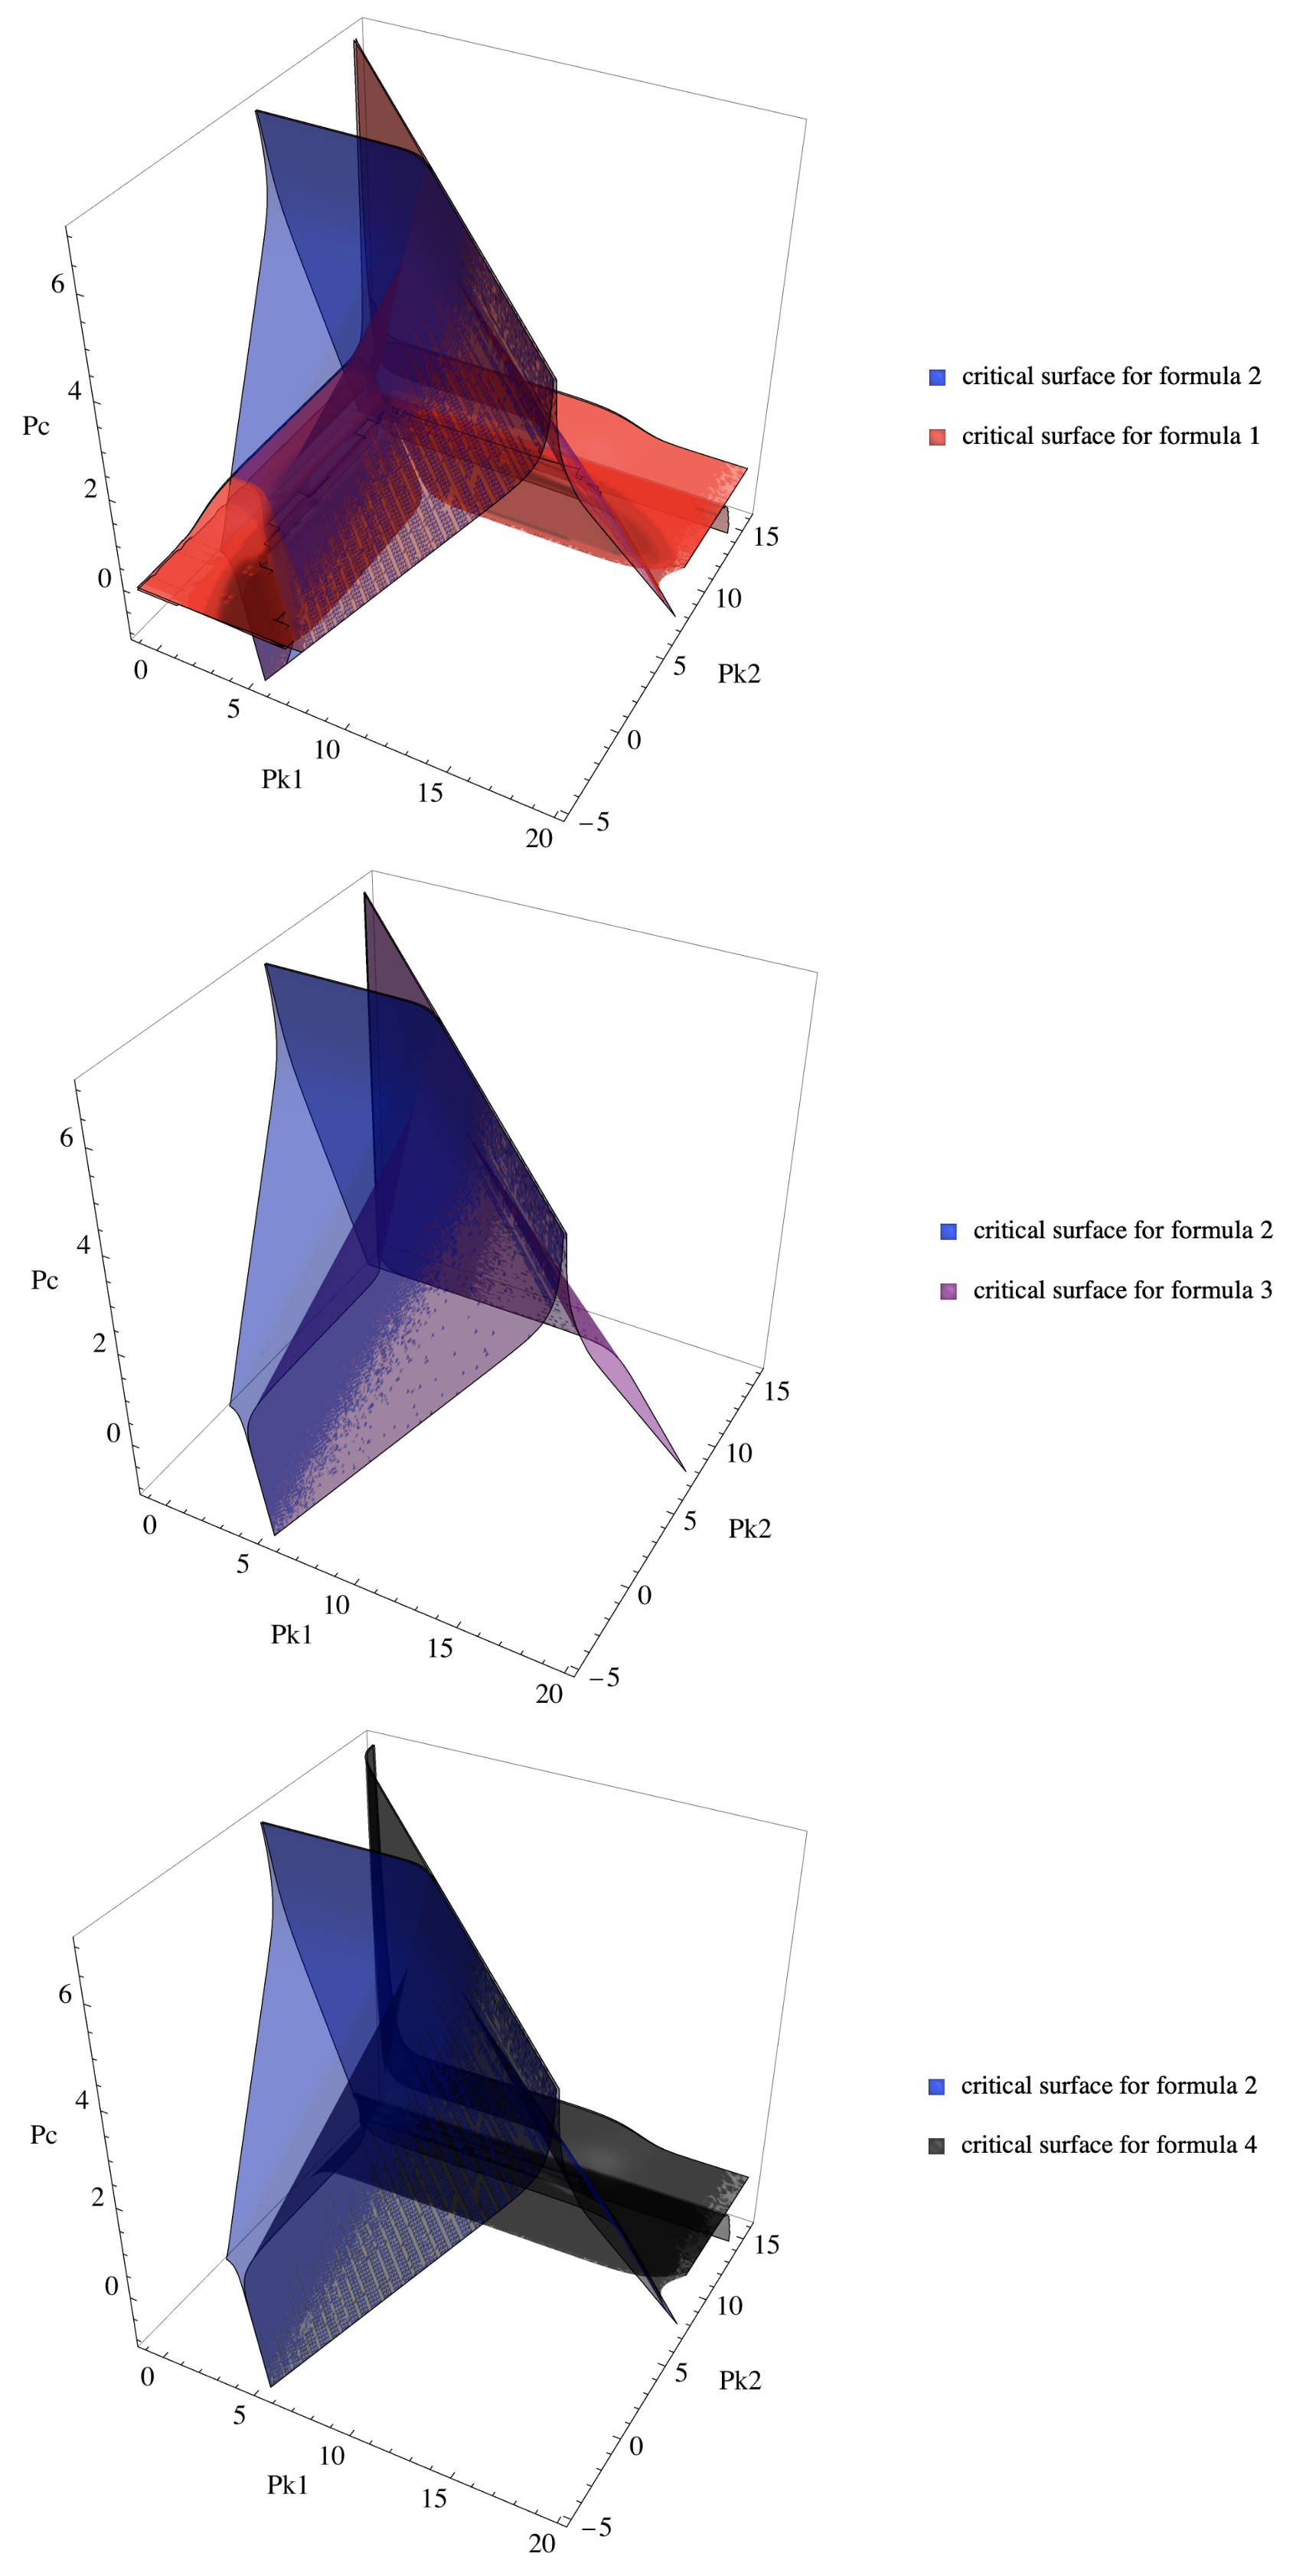
\includegraphics[width=0.7\textwidth]{重叠.png}
    \caption{\kaishu 可行域分别重叠}
    \label{fig:12}
\end{figure}

\end{document}
